\chapter{Results \& Evaluation} 

%How good is your solution? How well did you solve the general %problem, and what evidence do you have to support that?

%\section{Guidance}
%\begin{itemize}
%    \item
%        Ask specific questions that address the general problem.
%    \item
%        Answer them with precise evidence (graphs, numbers, %statistical
%        analysis, qualitative analysis).
%    \item
%        Be fair and be scientific.
%    \item
%        The key thing is to show that you know how to evaluate your %work, not
%        that your work is the most amazing product ever.
%\end{itemize}

This chapter will discuss data exploration findings and the predictive performances of our trained models.

\section{Data Exploration}

After creating our data set, we wanted to explore our classes' spread and the distributions of the chemical descriptors. This section also discusses the essential side effects and indications discovered.

\subsection{Principal Component Analysis (PCA)}

Principal component analysis is a dimensionality reduction method used to project data in a lower-dimensional space \citep{PCA}. We used it to project our chemical descriptor data for all drugs and compounds into a two-dimensional space in order to plot it and examine the spread of our two different classes.

Looking at Figure \ref{fig:PCA} we could see that BBB+ drugs and compounds were mostly closely packed together, with a few exceptions that appeared to be almost identical in some cases with drugs and compounds that are labelled as BBB-. These could be mislabelled drugs and compounds, but given the nature of the problem, we could not identify these with any confidence given our lack of medical and chemical knowledge. It could also be the case that these drugs and compounds could be using different methods to penetrate the blood-brain barrier, mentioned in Section \ref{sec:Motivation}, that are not accurately described just through their chemical properties.

BBB- drugs and compounds appeared to be more spread out with some very notable outliers that are later confirmed in Subsection \ref{subsec:CD_Ranges}


\begin{figure}[htb]
    \centering
    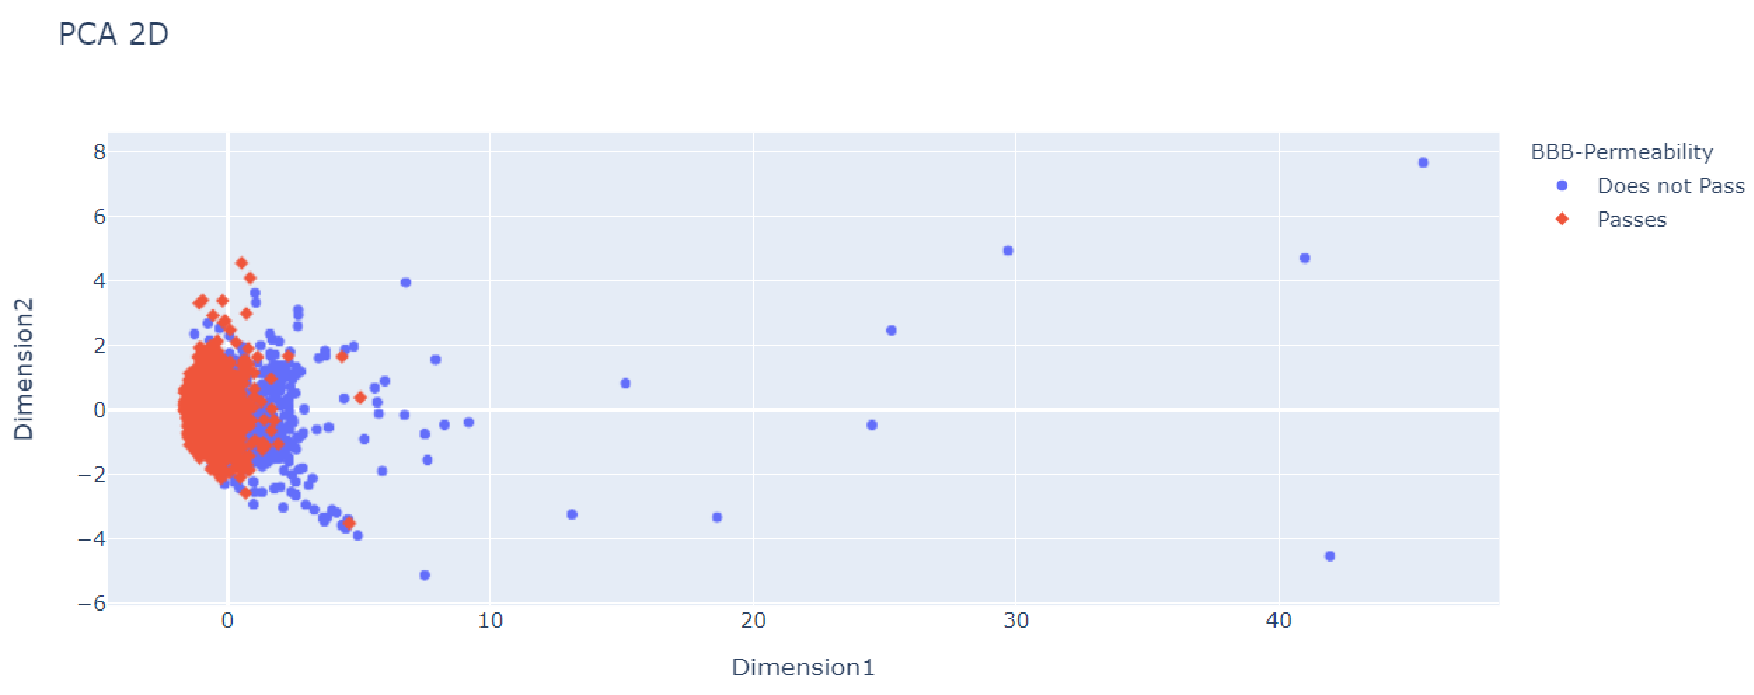
\includegraphics[width=1.0\linewidth]{images/PCA.pdf}    

    \caption{Principal component analysis plot after projecting the data set to a two-dimensional space.}

    \label{fig:PCA} 
\end{figure}


\subsection{Chemical Descriptors Ranges}
\label{subsec:CD_Ranges}

To explore our chemical descriptor data ranges, we decided to create violin plots combined with box plots.

It should be noted that the following discussion will explore the distributions found in our specific data set, a sample of drugs and compounds which may or may not be representative of the whole population of drugs and compounds that can penetrate the blood-brain barrier and of those that cannot.

Molecular Weight (MW) distribution, showcased by Figure \ref{fig:MW_Ranges}, showed that the greater number of drugs and compounds that could pass the blood-brain barrier had a MW in the range of 237.2-377.5. Whereas the majority of drugs and compounds that could not pass the blood-brain barrier had a MW in the range 318.4-539.6. A note should be made of the very large outliers appearing in the BBB- drugs and compounds, with a notable example having a MW of 7127. It appears that a smaller MW is preferable for BBB penetration. However, this is not always the case, as we can see BBB- drugs and compounds with a very low MW.

\begin{figure}[!ht]
    \centering
    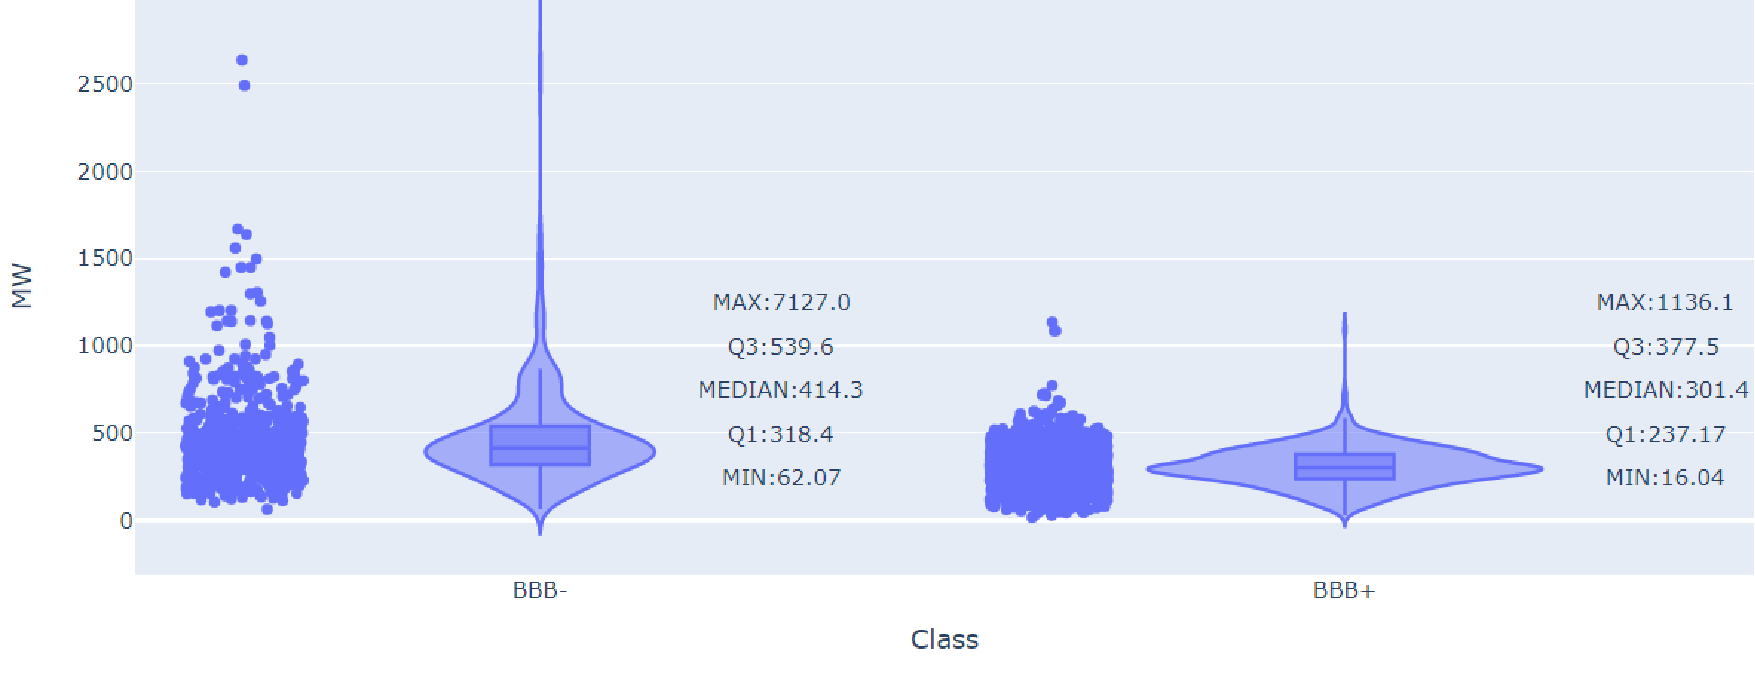
\includegraphics[width=0.9\linewidth]{images/MW Ranges.pdf}    

    \caption{Violin plots for the distribution of molecular weight (MW) values of each class}

    \label{fig:MW_Ranges} 
\end{figure}

Topological polar surface area (TPSA) distribution, showcased by Figure \ref{fig:TPSA_Ranges}, showed that the greater number of drugs and compounds that could pass the blood-brain barrier had a TPSA in the range of 32.3-74.6. Whereas the majority of drugs and compounds that could not pass the blood-brain barrier had a TPSA in the range 79.3-197. Again we can see some very large outliers in the BBB- drugs and compounds, with a notable example having a TPSA of 2860. Just as in the case of MW, it appears that a smaller TPSA is preferable.

\begin{figure}[!ht]
    \centering
    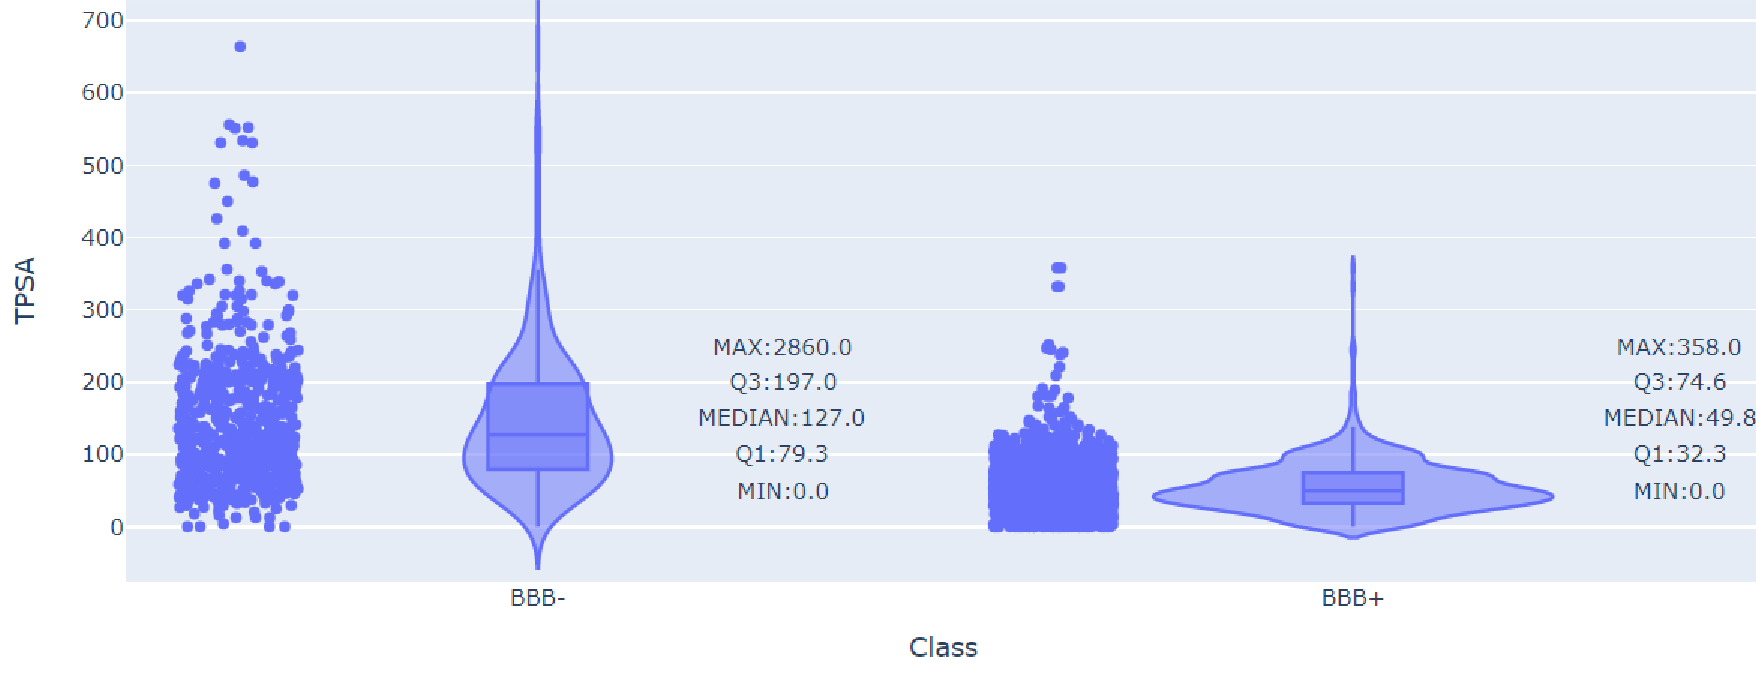
\includegraphics[width=0.9\linewidth]{images/TPSA Ranges.pdf}    

    \caption{Violin plots for the distribution of topological polar surface area (TPSA) values of each class}

    \label{fig:TPSA_Ranges} 
\end{figure}

Octanol-water partition coefficient (XLogP) distribution, showcased by Figure \ref{fig:XLogP_Ranges}, showed that the greater number of drugs and compounds that could pass the blood-brain barrier had an XLogP in the range of 1.6-3.8. Whereas the majority of drugs and compounds that could not pass the blood-brain barrier had an XLogP in the range -0.5-2.9. Again we can see some significant outliers in the BBB- drugs and compounds, with a notable example having an XLogP of -37.7. It seems that a small but positive XLogP is preferable.

\begin{figure}[!ht]
    \centering
    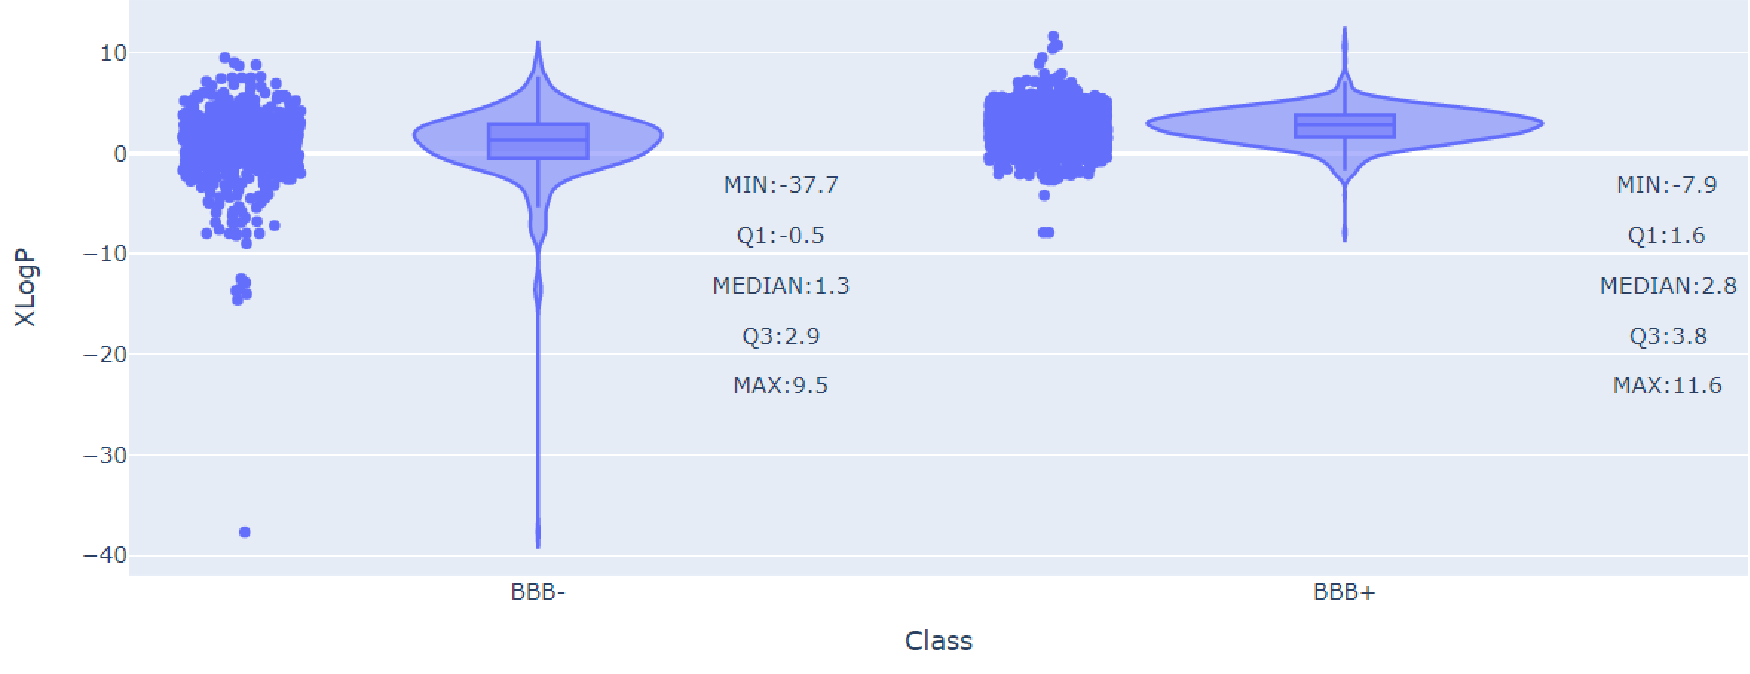
\includegraphics[width=0.9\linewidth]{images/XLogP Ranges.pdf}    

    \caption{Violin plots for the distribution of octanol-water partition coefficient (XLogP) values of each class}

    \label{fig:XLogP_Ranges} 
\end{figure}

Hydrogen-bond donors (NHD) distribution, showcased by Figure \ref{fig:NHD_Ranges}, showed that the greater number of drugs and compounds that could pass the blood-brain barrier had an NHD in the range of 0-2. Whereas the majority of drugs and compounds that could not pass the blood-brain barrier had an NHD in the range 2-4. Again we can see some significant outliers in the BBB- drugs and compounds, with a notable example having an NHD of 77. It seems that a smaller NHD is preferable.

\begin{figure}[!ht]
    \centering
    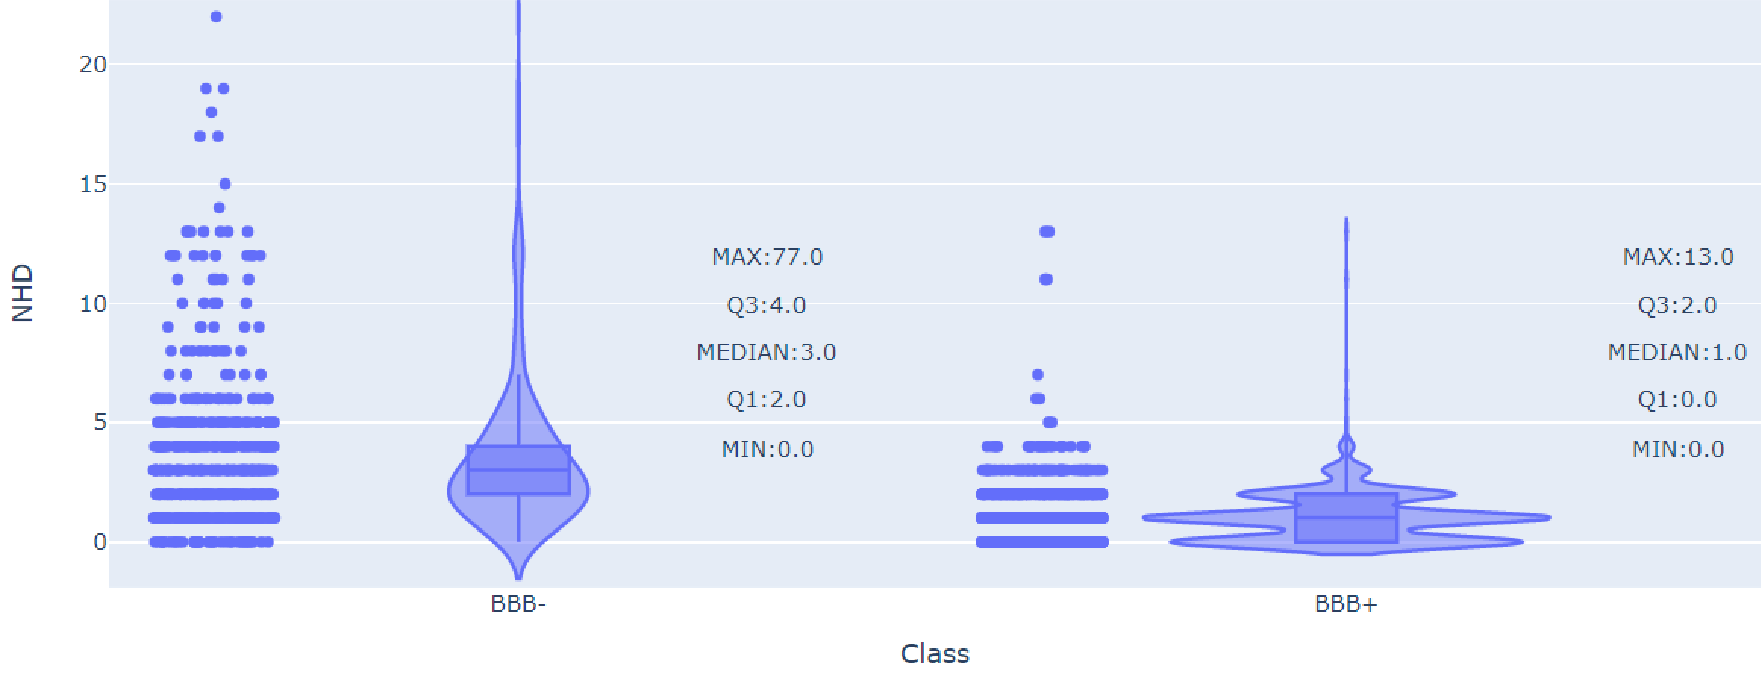
\includegraphics[width=0.9\linewidth]{images/NHD Ranges.pdf}    

    \caption{Violin plots for the distribution of the number of hydrogen-bond donors (NHD) of each class}

    \label{fig:NHD_Ranges} 
\end{figure}

Hydrogen-bond acceptors (NHA) distribution, showcased by Figure \ref{fig:NHA_Ranges}, showed that the greater number of drugs and compounds that could pass the blood-brain barrier had an NHA in the range of 2-5. Whereas the majority of drugs and compounds that could not pass the blood-brain barrier had an NHD in the range 5-11. Again we can see some significant outliers in the BBB- drugs and compounds, with a notable example having an NHA of 167. Just as in the case of NHD, it appears that a smaller NHA is preferable.

\newpage

\begin{figure}[!ht]
    \centering
    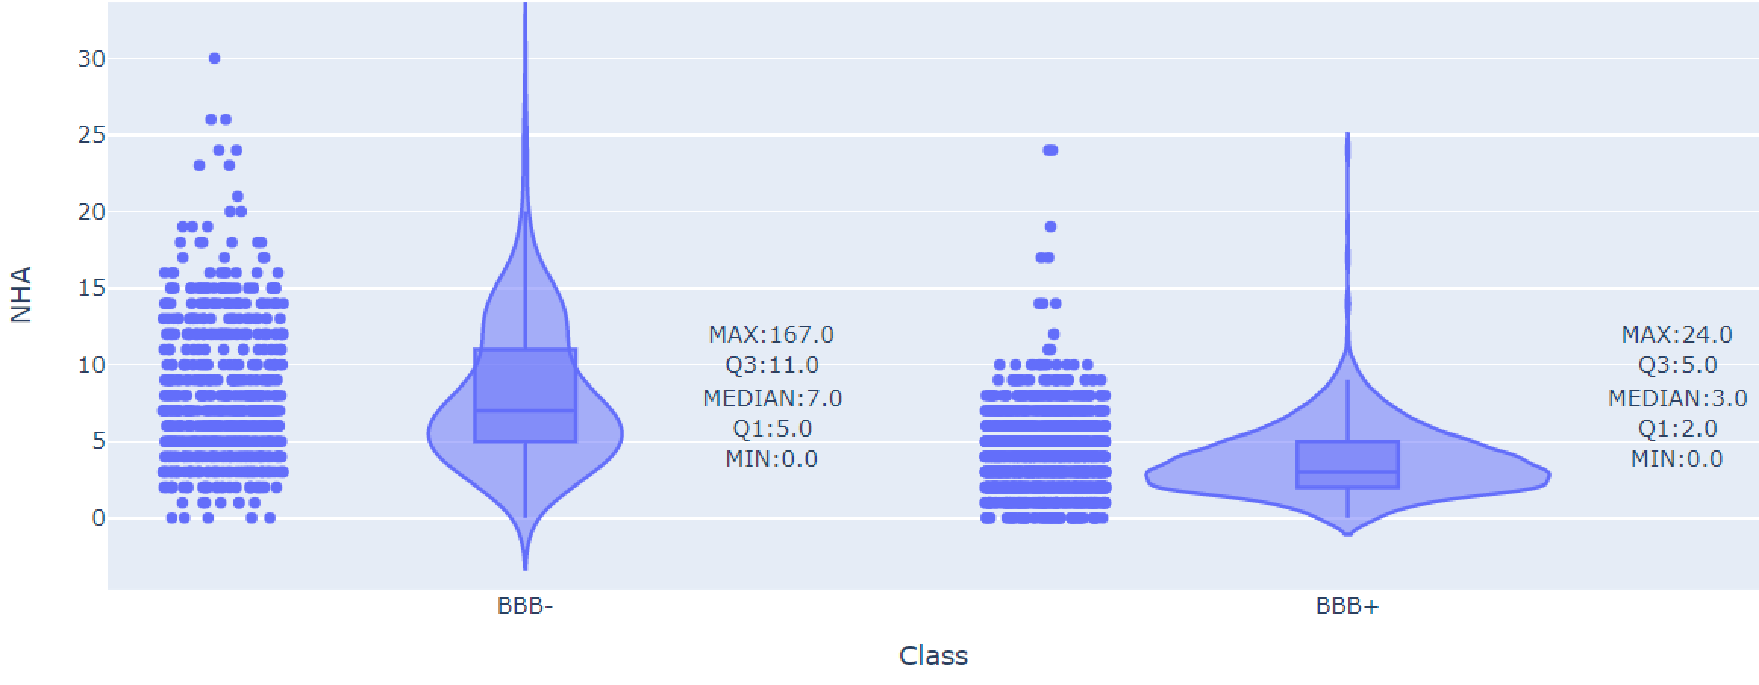
\includegraphics[width=0.9\linewidth]{images/NHA Ranges.pdf}    

    \caption{Violin plots for the distribution of the number of hydrogen-bond acceptors (NHA) of each class}

    \label{fig:NHA_Ranges} 
\end{figure}

The number of rotatable bonds (NRB) distribution, showcased by Figure \ref{fig:NRB_Ranges}, showed that the greater number of drugs and compounds that could pass the blood-brain barrier had an NRB in the range of 2-6. Whereas the majority of drugs and compounds that could not pass the blood-brain barrier had an NHD in the range 3-8. Again we can see some significant outliers in the BBB- drugs and compounds, with a notable example having an NRB of 178. Just as in the case of NHD and NHA, it appears that a smaller NRB is preferable. However, it is a bit unclear due to a considerable overlap between the two classes.

\begin{figure}[!ht]
    \centering
    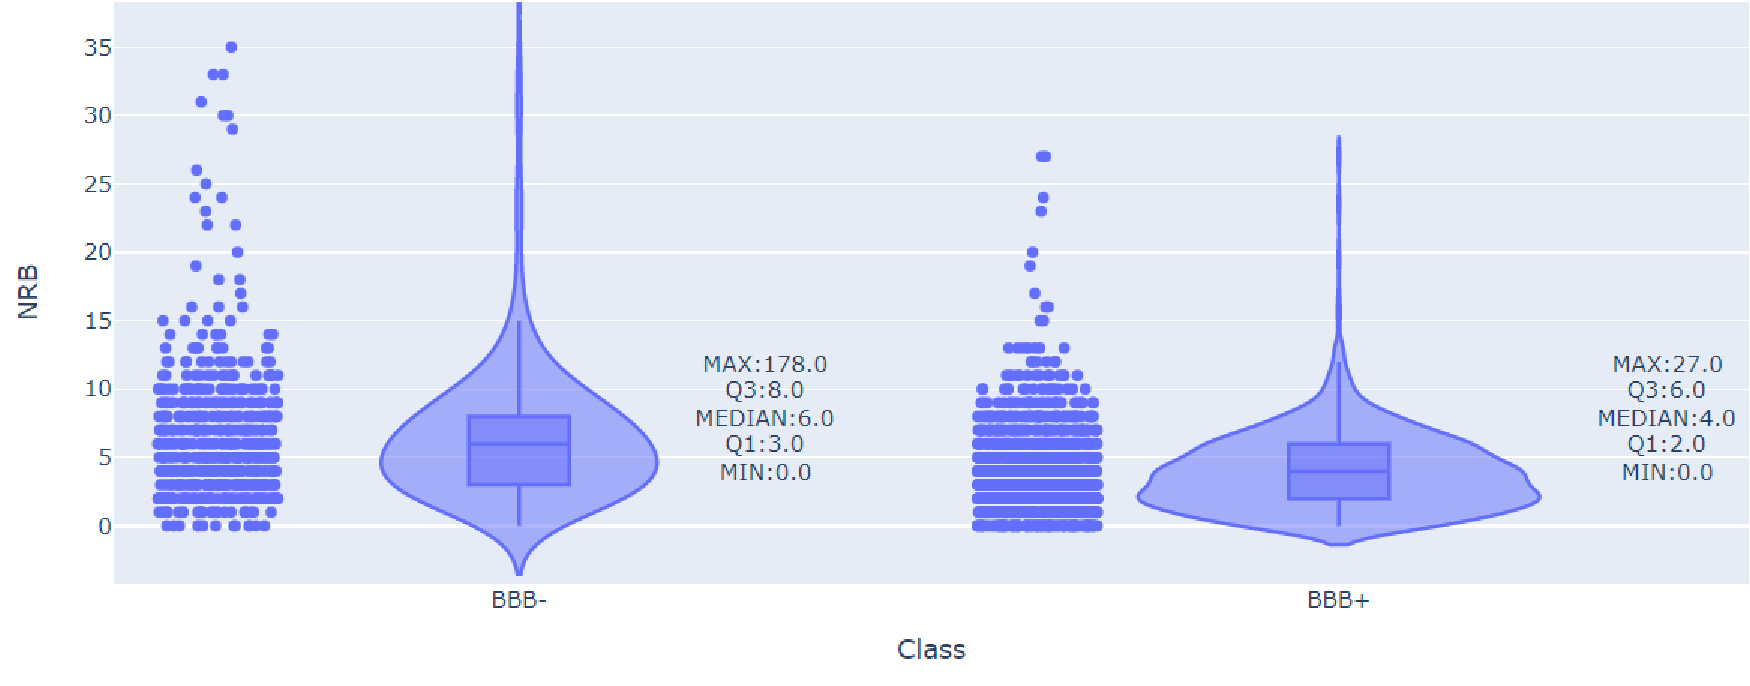
\includegraphics[width=0.9\linewidth]{images/NRB Ranges.pdf}    

    \caption{Violin plots for the distribution of the number of rotatable bonds (NRB) of each class}

    \label{fig:NRB_Ranges} 
\end{figure}

\subsection{Important Side Effects \& Indications}

As we have previously discussed in Subsection \ref{subsec:Classification_Models}, RFECV was used to primarily reduce the large number of side effects and indications used by some classification models. 

Table \ref{tbl:Side_Effects} showcases all the different side effects deemed highly important by RFECV. Some of them, such as depressed levels of consciousness or a coma, naturally seem sensible choices as they seem directly connected to the central nervous system. However, others, such as dry skin or influenza, seem less so.

Table \ref{tbl:Indications} showcases all the different indications deemed highly important by RFECV. In our opinion, all indications returned seem sensible.

\begin{table}[!ht]
  \caption{Top side effects according to RFECV. *Please ignore the <NA> entries, these were used as padding when creating the table.}
  \label{tbl:Side_Effects}
  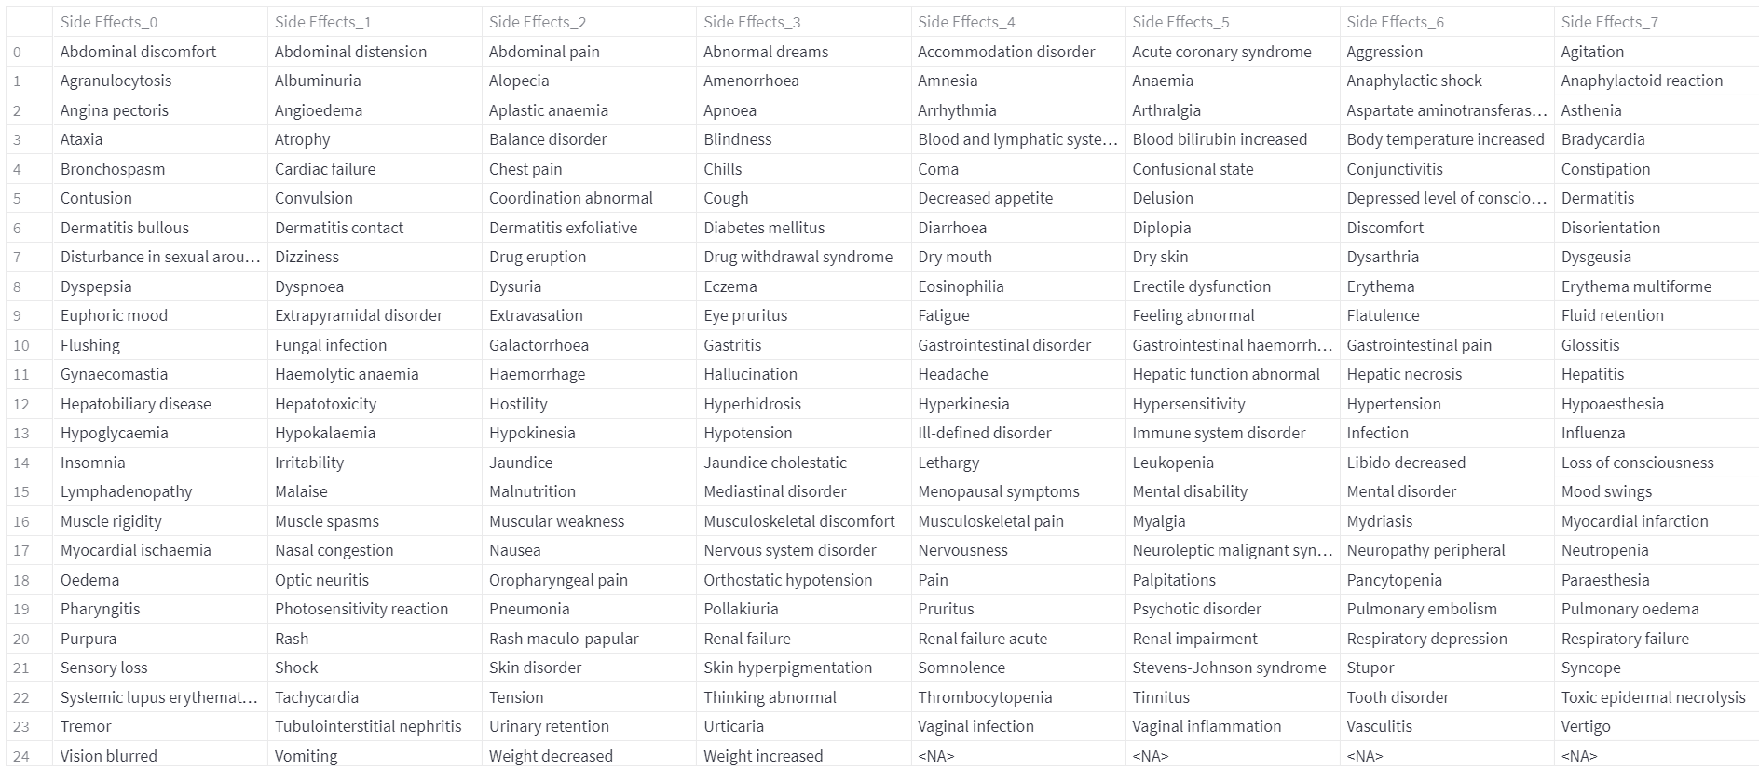
\includegraphics[width=1.0\linewidth]{images/Side Effects.pdf}
\end{table}

\begin{table}[!ht]
  \caption{Top indications according to RFECV.}
  \label{tbl:Indications}
  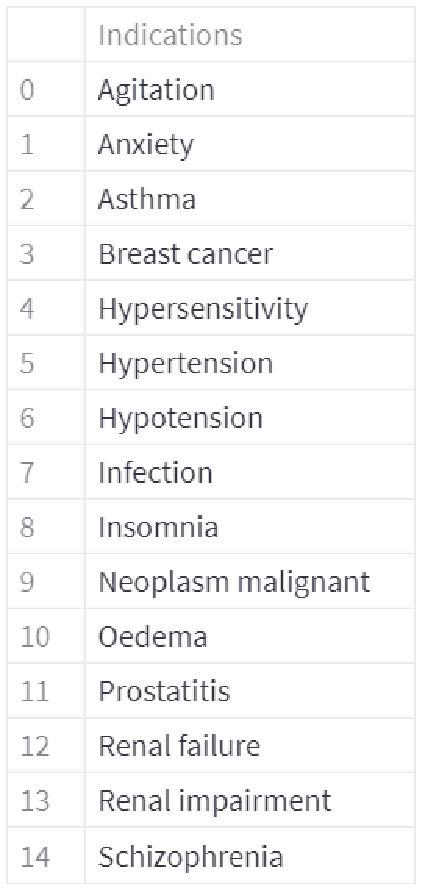
\includegraphics[width=0.2\linewidth]{images/Indications.pdf}
\end{table}


\section{Models Performance}

This section discusses the robustness and predictive performances of the different trained models and makes some comparisons.

\subsection{Classification Models Utilising Chemical Descriptors}
\label{subsec:Classification_CD}

Tables \ref{tbl:Classification_CD_Training} and \ref{tbl:Classification_CD_Testing} showcase the training and testing scores of all our classification models that only used chemical descriptors as their features. All of our models appear robust, with a permutation test p-value < 0.05, making them statistically significant. 

Even though six models were produced, excluding the Dummy Classifier, which is only used as a baseline, we would not recommend the use of the Logistic Regression and Support Vector Classification models. These models are only slightly better than the Dummy Classifier and have a very low MCC score, making them just marginally better than a coin flip.

Our best model seems to be the Random Forest Classifier, outperforming all the other models in every metric. A very close second would be the K-Nearest Neighbour Classifier.

\begin{table}
  \caption{Training performance of classification models with chemical descriptors used as features.}
  \label{tbl:Classification_CD_Training}
  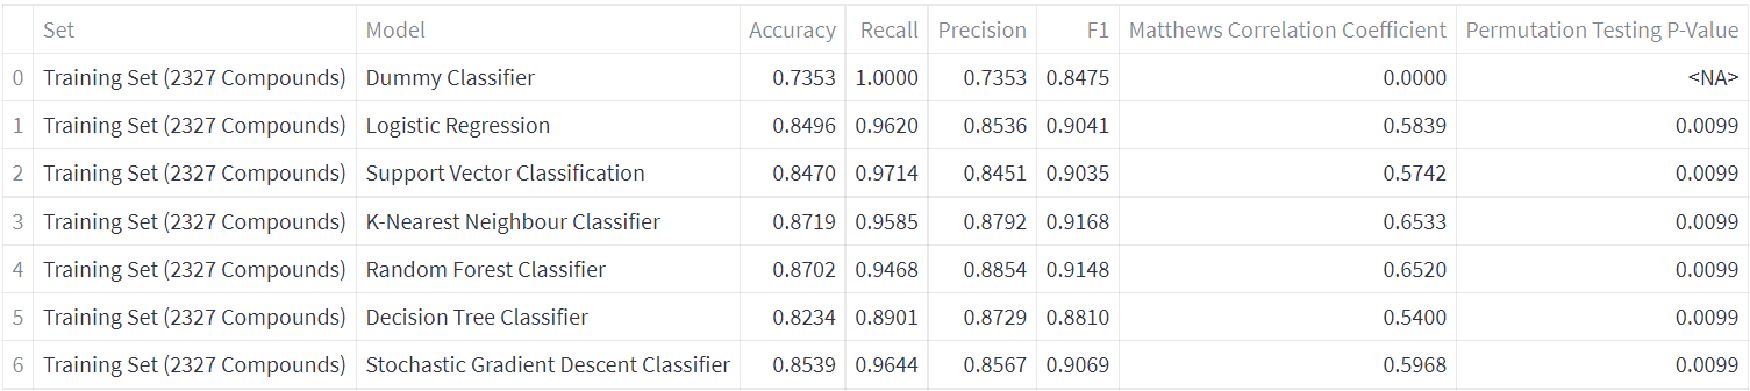
\includegraphics[width=1.0\linewidth]{images/Classification CD Training.pdf}
\end{table}

\begin{table}
  \caption{Testing performance of classification models with chemical descriptors used as features.}
  \label{tbl:Classification_CD_Testing}
  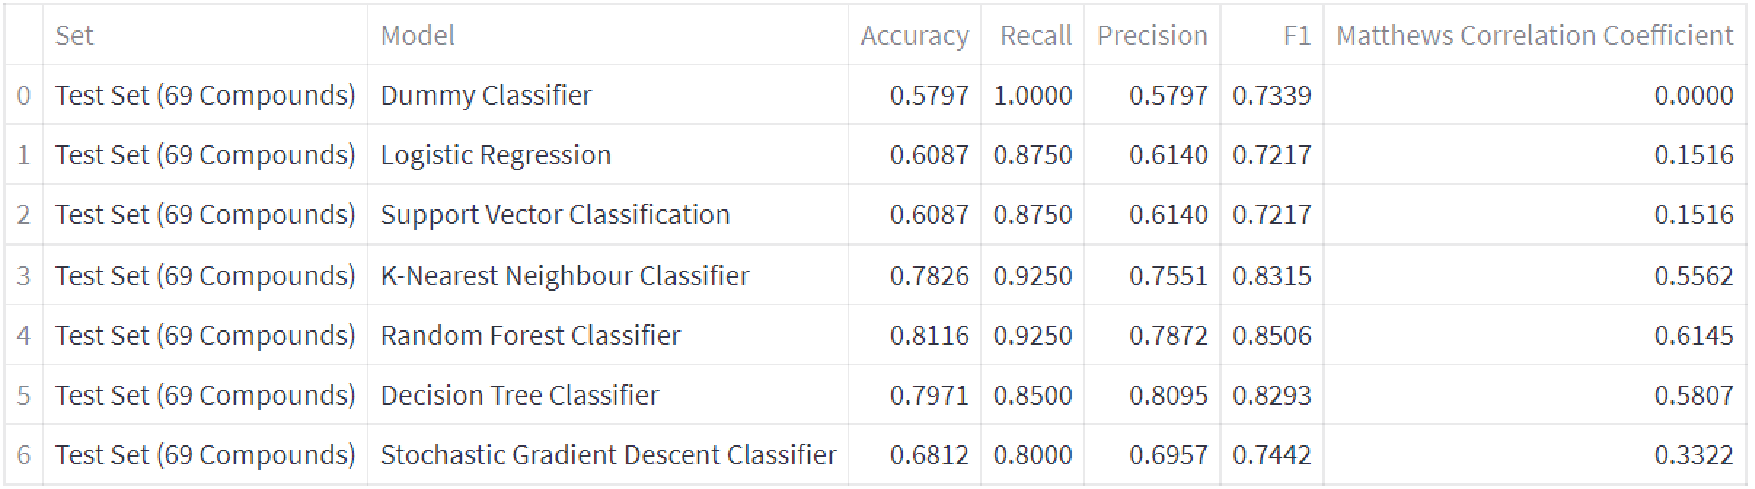
\includegraphics[width=1.0\linewidth]{images/Classification CD Testing.pdf}
\end{table}

\subsection{Classification Models Utilising Chemical Descriptors, Side Effects \& Indications}

Tables \ref{tbl:Classification_CD_SE_I_Training} and \ref{tbl:Classification_CD_SE_I_Testing} showcase the training and testing scores of all our classification models that used chemical descriptors, side effects and indications as their features. All of our models appear to be robust, with a permutation test p-value < 0.05, making them statistically significant. 

The addition of side effects and indications to the chemical descriptors appears to have substantially improved the performance of almost all models, except in the case of the Decision Tree Classifier, where its performance decreased.

Again, our best model seems to be the Random Forest Classifier, outperforming all the other models in every metric. A very close second would be the K-Nearest Neighbour Classifier.

\begin{table}[!ht]
  \caption{Training performance of classification models with chemical descriptors, side effects and indication used as features.}
  \label{tbl:Classification_CD_SE_I_Training}
  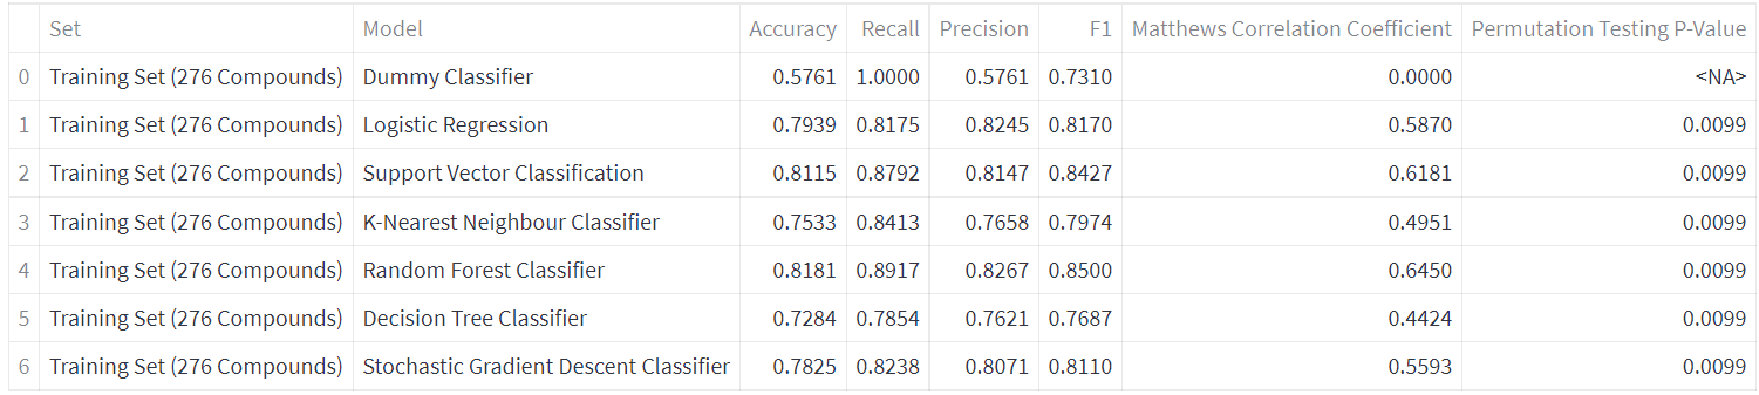
\includegraphics[width=1.0\linewidth]{images/Classification CD SE I Training.pdf}
\end{table}

\newpage

\begin{table}[!ht]
  \caption{Testing performance of classification models with chemical descriptors, side effects and indication used as features.}
  \label{tbl:Classification_CD_SE_I_Testing}
  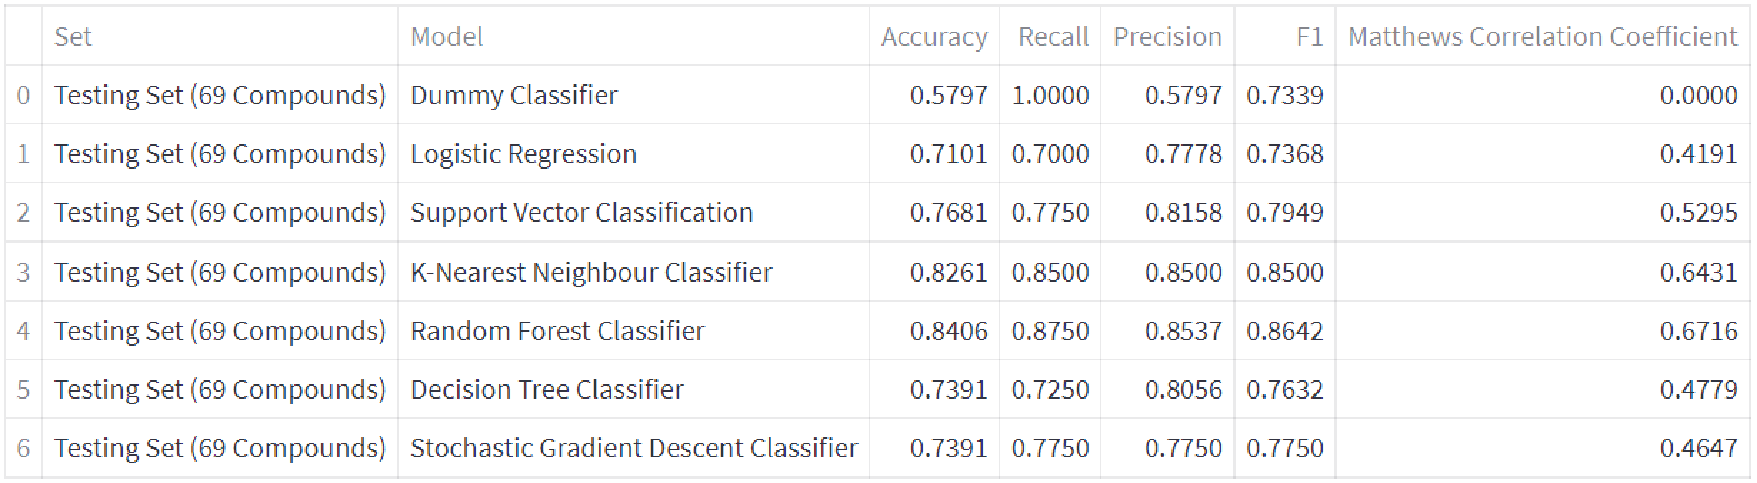
\includegraphics[width=1.0\linewidth]{images/Classification CD SE I Testing.pdf}
\end{table}

\subsection{Regression Models Utilising Chemical Descriptors}

Tables \ref{tbl:Regression_CD_Training} and \ref{tbl:Regression_CD_Testing} showcase the training and testing scores of all our regression models that only used chemical descriptors as their features. All of our models, except the Decision Tree Regressor, appear to be robust, with a permutation test p-value < 0.05, making them statistically significant. 

Our best model seems to be the Support Vector Regression, outperforming all the other models in every metric.

\begin{table}[!ht]
  \caption{Training performance of regression models with chemical descriptors used as features.}
  \label{tbl:Regression_CD_Training}
  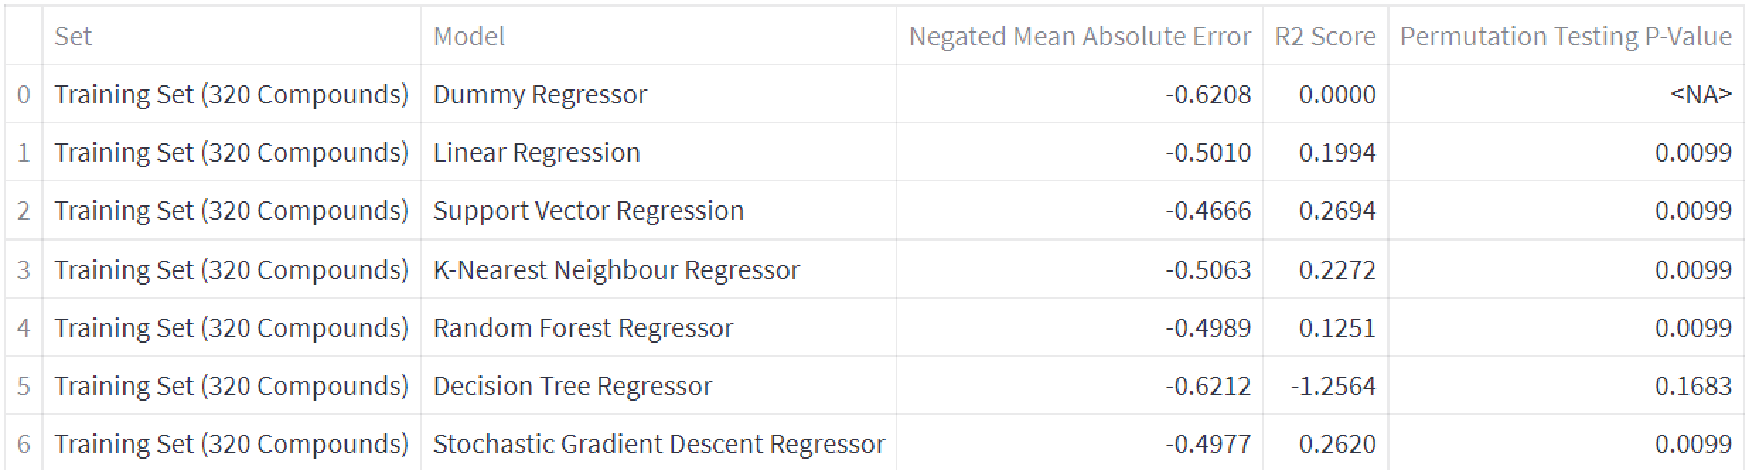
\includegraphics[width=1.0\linewidth]{images/Regression CD Training.pdf}
\end{table}

\begin{table}[!ht]
  \caption{Testing performance of regression models with chemical descriptors used as features.}
  \label{tbl:Regression_CD_Testing}
  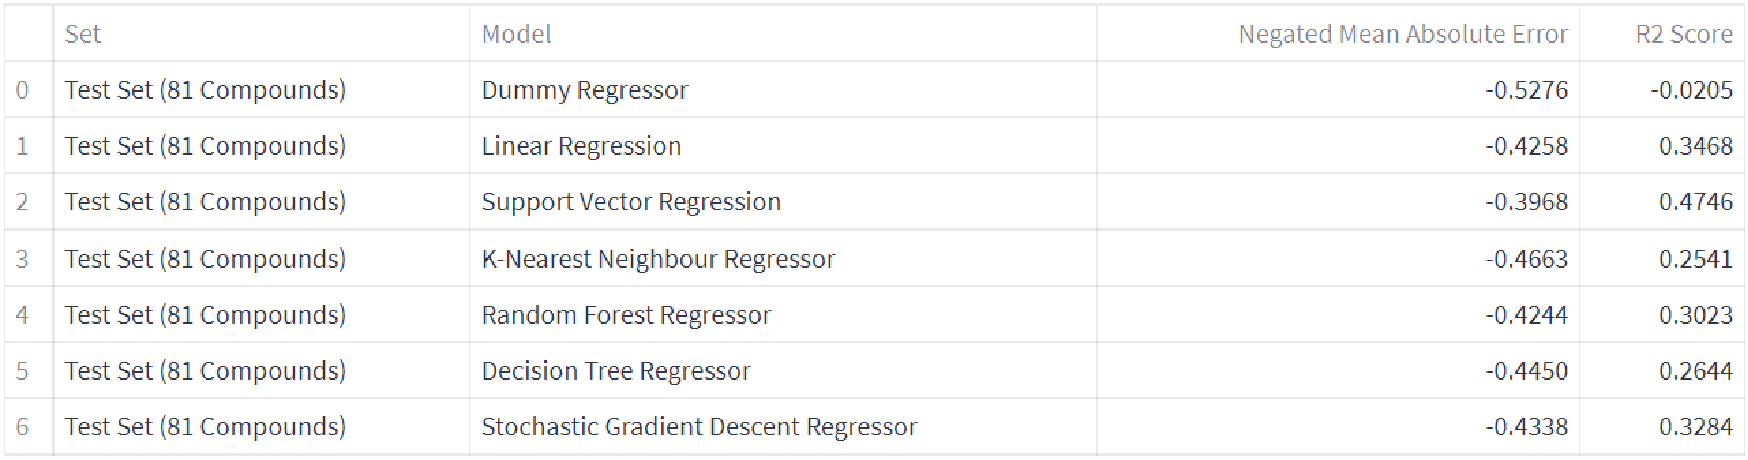
\includegraphics[width=1.0\linewidth]{images/Regression CD Testing.pdf}
\end{table}

\section{Project Evaluation}

All objectives specified in Section \ref{sec:Objectives} were successfully achieved. 

We managed to create a substantial data set that was used to create both classification and regression models using a very small number of chemical descriptors, further confirming the conclusions reached by \citet{Zhao2007, Saber2020} that models predicting the blood-brain barrier permeability of drugs and compounds can be built using a minimal number of hydrogen-bonding chemical descriptors. All of our models, except for a single one, were statistically significant however some were only marginally better than a coin flip as discussed in Subsection \ref{subsec:Classification_CD}

The project also managed to validate the conclusion reached by \cite{Gao2017} that the addition of side effects and indications to chemical descriptors substantially improved the predictive performance of models. All but one of our classification models' predictive performances improved by adding side effects and indications, even though we used a different technique and a smaller number of chemical descriptors. Our Random Forest Classifier even achieved somewhat similar performance to the Support Vector Machine trained by \citet{Gao2017}, showcased by Table \ref{tbl:Gao_Model_Comparison}.